\documentclass[journal]{IEEEtran}

\usepackage[T1]{fontenc}
\usepackage[utf8]{inputenc}
\usepackage{amsmath,amssymb,amsfonts}
\usepackage{graphicx}
\usepackage{booktabs}
\usepackage{array}
\usepackage{url}
\usepackage{xcolor}
\usepackage[hidelinks]{hyperref}
\usepackage{orcidlink}
\usepackage{balance}

\graphicspath{{../figures/}}

\renewcommand{\topfraction}{0.92}
\renewcommand{\bottomfraction}{0.75}
\renewcommand{\textfraction}{0.08}
\renewcommand{\floatpagefraction}{0.80}

% IEEEtran hard-codes an em-dash after the abstract and index-terms names; the CAOS
% content standard (ADR-0067) excludes em-dashes, so the separator is a full stop.
\makeatletter
\def\abstract{\normalfont
    \if@twocolumn
      \@IEEEabskeysecsize\bfseries\textit{\abstractname}.\ \relax
    \else
      \bgroup\par\addvspace{0.5\baselineskip}\centering\vspace{-1.78ex}\@IEEEabskeysecsize\textbf{\abstractname}\par\addvspace{0.5\baselineskip}\egroup\quotation\@IEEEabskeysecsize
    \fi\@IEEEgobbleleadPARNLSP}
\def\IEEEkeywords{\normalfont
    \if@twocolumn
      \@IEEEabskeysecsize\bfseries\textit{\IEEEkeywordsname}.\ \relax
    \else
      \bgroup\par\addvspace{0.5\baselineskip}\centering\@IEEEabskeysecsize\textbf{\IEEEkeywordsname}\par\addvspace{0.5\baselineskip}\egroup\quotation\@IEEEabskeysecsize
    \fi\@IEEEgobbleleadPARNLSP}
\makeatother

% Page-1 header block (conventions/manuscript-header-standard.md). The four document
% macros are set by the publishing tool when the version DOI is reserved.
\newcommand{\doctype}{Technical report}
\newcommand{\docversion}{v2.2}
\newcommand{\docdate}{18 September 2026}
\newcommand{\versiondoi}{10.5281/zenodo.22834763}
\newcommand{\conceptdoi}{10.5281/zenodo.21519687}
\newcommand{\docrepo}{github.com/fsantibanezleal/CAOS\_PitForge}
\newcommand{\headerblock}{%
\begin{center}
\fbox{\parbox{0.94\textwidth}{\small\raggedright
\textbf{\doctype} \quad$\cdot$\quad \docversion, \docdate \quad$\cdot$\quad Licence CC BY 4.0\\[2pt]
CAOS open-research programme \quad$\cdot$\quad CAOS\_PitForge, open-pit design optimisation\\[2pt]
Version DOI \href{https://doi.org/\versiondoi}{\texttt{\versiondoi}} \quad$\cdot$\quad
concept DOI (always latest) \href{https://doi.org/\conceptdoi}{\texttt{\conceptdoi}}\\[2pt]
Not peer reviewed. Source code, data and computational records: \href{https://\docrepo}{\texttt{\docrepo}}
}}
\end{center}}

\begin{document}

\title{PitForge: Exact Ultimate-Pit Optimization\\ Reproducing the Published MineLib Optima,\\ with Whittle Nested Shells and Scheduling}

\author{Felipe~Santib\'a\~nez-Leal~\orcidlink{0000-0002-0150-3246}%
\thanks{F. Santib\'a\~nez-Leal is with the CAOS open-research programme, Santiago, Chile
(e-mail: fsantibanez@gmail.com; ORCID 0000-0002-0150-3246).}%
\thanks{Interactive tool and reproducible pipeline (MIT) at
\url{https://github.com/fsantibanezleal/CAOS_PitForge}; the tool is available at
\url{https://pitforge.fasl-work.com}.}}

% The leading {} lets IEEEtran's \MakeUppercase reach \doctype, so the whole head is set in capitals.
\markboth{{}\doctype\ \docversion, 2026}%
{Santib\'a\~nez-Leal: Exact ultimate-pit optimization with nested shells and scheduling}

\IEEEaftertitletext{\vspace{-0.6\baselineskip}\headerblock\vspace{0.2\baselineskip}}

\maketitle

\begin{abstract}
The first optimization of open-pit mine design is the ultimate pit limit: given a block model in which each block
carries a net economic value and a set of slope-precedence constraints, find the set of blocks to extract that
maximises total value while respecting the slopes. The problem has an exact polynomial solution as the
maximum-weight closure of the precedence graph, computed as a minimum cut. PitForge implements it in a TypeScript
engine that also runs in the browser, where the pit is re-solved as the price, revenue factor or slope change,
validates the solver against published optima, and extends it to the two decisions that follow. On the three of
MineLib's eleven instances that have a verified public mirror (newman1, zuck\_small and kd, $1060$ to $14153$
blocks), the solver reproduces the \emph{published} optimum to a relative error of $10^{-9}$ or less, and an
independent pseudoflow solver returns the same values. Beyond the single pit, the tool computes the Whittle nested
pit shells, the family of optimal pits over an ascending revenue-factor schedule, with the value, tonnage and
strip-ratio curves that guide phase and pushback design, and it solves two separate constrained
production-scheduling scenarios. On the published \texttt{newman1.cpit} scenario (six periods, $8\%$ discount and
two resources), it reproduces the published $24{,}486{,}184$ LP bound and finds a feasible $23{,}553{,}245$
heuristic schedule, a $3.81\%$ gap. A separate synthetic twin (eight periods, $10\%$ discount and one resource) has
an $11.29\%$ gap and is not comparable. Every pit value is checked against the flow identity
$\text{pit value} = \sum\text{positive value} - \text{max flow}$ on every solve.
\end{abstract}

\begin{IEEEkeywords}
Open-pit mining, ultimate pit limit, maximum closure, minimum cut, maximum flow, nested pit shells, Whittle,
production scheduling, MineLib.
\end{IEEEkeywords}

\section{Introduction}

\IEEEPARstart{T}{he} ultimate pit limit (UPL) is the foundational optimization of open-pit mine design: given a
three-dimensional block model in which each block has a net value (recoverable metal less mining and processing
cost) and slope-precedence constraints (a block can be mined only after those above it in the pit wall), which set
of blocks maximises total value? The problem has an exact, polynomial-time solution, established by Lerchs and
Grossmann~\cite{lg} and understood through Picard's theorem~\cite{picard} as the maximum-weight closure of the
precedence graph, which is the source side of a minimum $s$--$t$ cut and hence solvable by any maximum-flow
algorithm~\cite{fordfulkerson,hochbaum}. This is textbook operations research~\cite{newman}; what a practical tool
adds is validation against known answers, the family of nested pits used for phase design, and the connection to
the production schedule.

PitForge solves the UPL as a minimum cut and checks the value identity on every solve. It is validated here
against the published MineLib benchmark optima~\cite{minelib}, and it extends the exact solve to the Whittle
nested pit shells~\cite{whittle}, the optimal pits across an ascending revenue factor that give the
value-tonnage-strip curves phase design rests on, and to a constrained production schedule~\cite{chicoisne}, for
which it reports the gap to a certified bound. The contribution is an exact, validated implementation that
reproduces the literature and states where exactness ends, not a new algorithm.

\section{The Exact Pit, Validated on MineLib}\label{sec:minelib}

\begin{figure*}[!t]
\centering
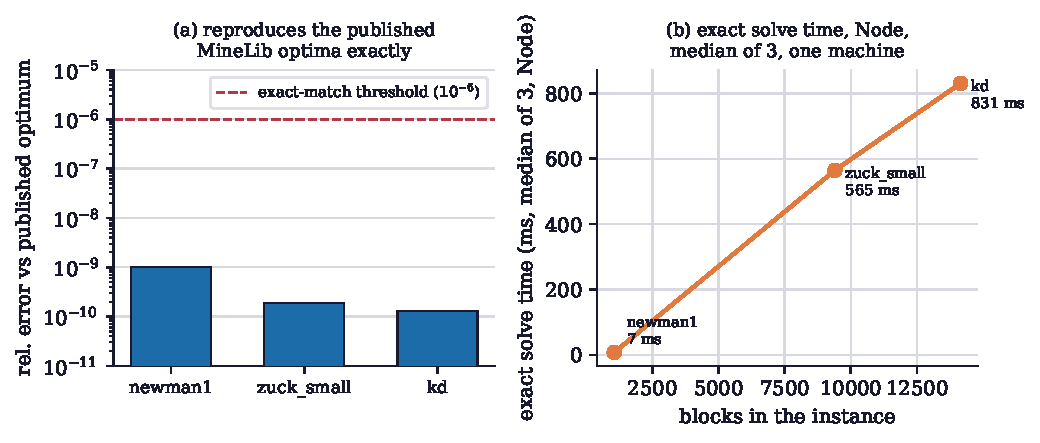
\includegraphics[width=0.86\textwidth]{fig-minelib.pdf}
\caption{Validation on the public MineLib instances. \textbf{(a)} The solver reproduces the \emph{published}
optimum of newman1, zuck\_small and kd to a relative error of $10^{-9}$ or less. \textbf{(b)} Exact solve time
against instance size, measured under Node on one machine as the median of three runs: milliseconds for the
$1060$-block newman1 and under a second for the $14153$-block kd. These are timings of one environment, not a
property of the method; repeat runs on the same machine varied by a factor of two to five, and the artifact
records the environment beside them. The browser runs the same engine and displays its own measured time; the
figure plots the Node measurements.}
\label{fig:minelib}
\end{figure*}

The ultimate pit is the maximum-weight closed set of the precedence graph, and PitForge computes it by Picard's
reduction to a minimum cut: a source arc to every positive-value block, a sink arc from every negative block, and
an infinite-capacity arc for each precedence relation, after which a Dinic maximum flow~\cite{dinic} gives the pit
as the source-reachable set. The closure property and the value identity
$\text{pit value} = \sum_{v_b>0} v_b - \text{maxflow}$ are asserted on every solve, so an inconsistent value
cannot be returned without an error. The validation uses three of MineLib's eleven instances, those with a verified
public mirror (Fig.~\ref{fig:minelib}, Table~\ref{tab:minelib}); the other eight, among them marvin and the
McLaughlin instances, lack a verified mirror or, for mclaughlin, its precedence file. On all three, PitForge's value matches the published optimum to a relative error of
$9.96\times10^{-10}$ on newman1, $1.86\times10^{-10}$ on zuck\_small and $1.30\times10^{-10}$ on kd, which is
agreement to floating-point precision, and an independent pseudoflow solver~\cite{hochbaum} returns the same value on
each. Under Node, running the same TypeScript engine the browser runs, the $1060$-block newman1 solves in
milliseconds and the $14153$-block kd in under a second. Those times are machine-dependent, so no decimal figure is
quoted; within one run, the pseudoflow solver is one to two orders of magnitude slower than Dinic on the two larger
instances.

\begin{table}[!t]
\centering
\caption{PitForge versus the published MineLib optima. The solver matches all three to a relative error of
$10^{-9}$ or less. Solve times are omitted because they are machine-dependent; the artifact records them with the
environment they were measured in.}
\label{tab:minelib}
\footnotesize
\begin{tabular}{@{}l r r r@{}}
\toprule
Instance & blocks & published optimum & rel. error \\
\midrule
newman1    & $1060$  & $2.6087\times10^{7}$ & $1.0\times10^{-9}$ \\
zuck\_small & $9400$  & $1.4227\times10^{9}$ & $1.9\times10^{-10}$ \\
kd         & $14153$ & $6.5220\times10^{8}$ & $1.3\times10^{-10}$ \\
\bottomrule
\end{tabular}
\end{table}

\section{Nested Shells and Scheduling}\label{sec:whittle}

\begin{figure*}[!t]
\centering
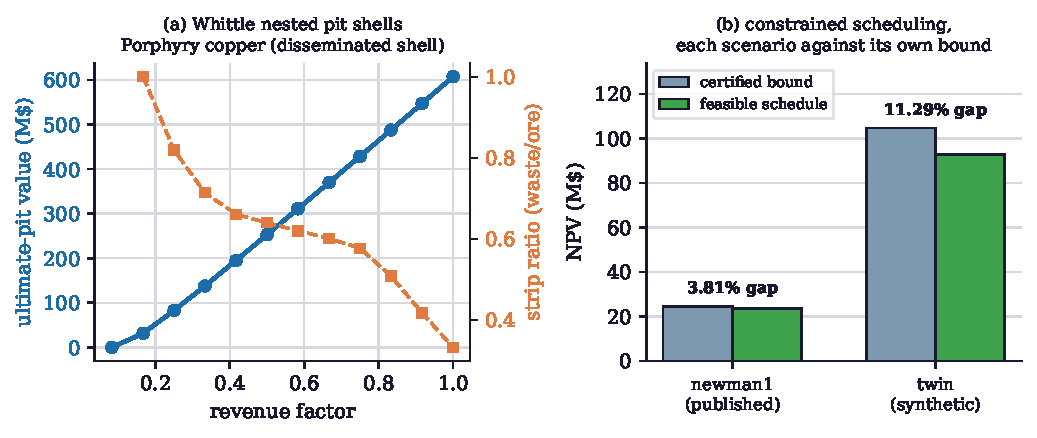
\includegraphics[width=0.86\textwidth]{fig-whittle.pdf}
\caption{Beyond the single pit. \textbf{(a)} The Whittle nested pit shells of a porphyry copper case: solving the
ultimate pit over an ascending revenue factor gives a family of nested pits whose value rises and whose strip ratio
falls as the pit grows. The first shell is empty, since no block pays for itself at that revenue factor, so the
value curve starts at zero, and the strip-ratio series, which is waste over ore and therefore undefined without ore,
starts at the second shell. \textbf{(b)} The two constrained-scheduling scenarios, each against its own relaxation
bound. Left, the published \texttt{newman1.cpit} scenario, six periods at $8\%$ discount with two resource
constraints: a certified upper bound of $24.49$ million against a feasible greedy schedule of $23.55$ million, a
$3.81\%$ gap, with the bound reproducing MineLib's published LP bound to $3.7\times10^{-9}$. Right, a separate
synthetic twin, eight periods at $10\%$ discount with one movement limit: $104.6$ million against $92.8$ million, an
$11.29\%$ gap. The two gaps have different denominators and are not one number.}
\label{fig:whittle}
\end{figure*}

A mine is not designed as one pit but as a sequence, and PitForge computes the two objects that sequence rests on
(Fig.~\ref{fig:whittle}). The first is the Whittle nested pit shells~\cite{whittle}: solving the ultimate pit over
an ascending schedule of revenue factors (multiplying the metal price) yields a family of nested optimal pits, from
the first non-empty pit at a revenue factor of $0.17$ to the full pit at a factor of one, and their value, tonnage
and strip-ratio curves (Fig.~\ref{fig:whittle}a) are what a planner uses to choose phases and pushbacks. Because
each shell is an exact ultimate-pit solve, the whole family is exact. The second is the production schedule:
assigning the pit's blocks to time periods under capacity constraints to maximise discounted value is the
constrained pit scheduling problem~\cite{chicoisne}, harder than the UPL. PitForge bounds it with the linear
relaxation of the time-indexed formulation and builds a feasible schedule with an independent greedy heuristic, not
a rounding of the relaxation, and reports the gap between the two (Fig.~\ref{fig:whittle}b). On the published
\texttt{newman1.cpit} definition (six periods, $8\%$ discount, total-movement and processing limits) it reproduces
the $24{,}486{,}184$ bound to a relative error of $3.7\times10^{-9}$ and finds a feasible $23{,}553{,}245$ schedule,
a $3.81\%$ gap to that bound. MineLib's cited historical feasible value is $23{,}483{,}671$, a $4.1\%$ gap; the
heuristic exceeds it by $0.30\%$, and no comparison with later published schedules is made here, so no best-known
result is claimed. The synthetic-twin scenario has a $104.6$~million bound and a $92.8$~million feasible schedule,
an $11.29\%$ gap. The two scenarios have different denominators, and each gap is stated with its scenario.

\section{Discussion and Scope}\label{sec:discuss}

The ultimate pit and the nested shells are solved \emph{exactly}, and the reproduction of the MineLib optima to
relative error $10^{-9}$ or less validates the implementation; the schedule is solved to a certified bound with the
gap reported, because the scheduling problem, unlike the UPL, does not admit a cheap exact solve at these sizes. The
value identity checked on every solve guarantees that a returned pit value is consistent with the computed flow.
The validation covers three MineLib instances of up to $14153$ blocks; the other eight, all larger ($29277$ to
$2.1$ million blocks), are not attempted. MineLib is licensed CC BY-SA 3.0 Unported; source instances are fetched at run time
and only attributed summary numbers (the optima and timings) are kept in the repository. The synthetic cases used
for the nested shells and the schedule are physically reasonable block models, not a specific deposit, so their
numbers illustrate the method rather than predict a mine. The tool computes the pit and the schedule; it does not
replace the geological, geotechnical and financial judgement that turns them into a mine plan.

\section{Conclusion}

PitForge solves the open-pit ultimate pit limit exactly, as a maximum-closure minimum cut, and reproduces the three
published MineLib optima with a verified public mirror to a relative error of $10^{-9}$ or less, with an independent
pseudoflow solver agreeing. It extends the exact solve to the Whittle nested pit shells that guide phase design, and
to constrained production scheduling, whose gap to a certified bound it reports per scenario: $3.81\%$ for the
published \texttt{newman1.cpit} scenario and $11.29\%$ for a separate, non-comparable synthetic twin.

\appendices
\section{Reproduction}\label{app:repro}

The repository artifacts under \path{data/derived/} carry the MineLib benchmark (\path{minelib-results.json}:
per-instance published optimum, solved value, relative error, the Dinic and pseudoflow timings and the timing
environment), the nested-shell curves per case (\path{case-results.json}: revenue factor, pit value, tonnage and
strip ratio), and the constrained schedules (\path{cpit-schedule.json}: the certified LP bound and the net present
value of the greedy schedule per scenario). The figure script under \path{manuscripts/ultimate-pit/figures/} reads
those artifacts directly and writes the plotted values to \path{manuscripts/ultimate-pit/data/pf.json}. The exact
solver is deterministic, so re-running reproduces Table~\ref{tab:minelib} and Figs.~\ref{fig:minelib}
and~\ref{fig:whittle}, except for the machine-dependent timings. The MineLib instances are CC BY-SA 3.0 Unported and
are fetched from public mirrors into a local cache that is not kept in the repository.

\balance

\begin{thebibliography}{00}

\bibitem{lg} H.~Lerchs and I.~F. Grossmann, ``Optimum design of open-pit mines,'' \emph{CIM Bulletin},
vol.~58, pp.~47--54, 1965.

\bibitem{picard} J.-C. Picard, ``Maximal closure of a graph and applications to combinatorial problems,''
\emph{Management Science}, vol.~22, no.~11, pp.~1268--1272, 1976. doi:10.1287/mnsc.22.11.1268.

\bibitem{fordfulkerson} L.~R. Ford and D.~R. Fulkerson, ``Maximal flow through a network,'' \emph{Canadian
Journal of Mathematics}, vol.~8, pp.~399--404, 1956. doi:10.4153/CJM-1956-045-5.

\bibitem{hochbaum} D.~S. Hochbaum, ``The pseudoflow algorithm: A new algorithm for the maximum-flow problem,''
\emph{Operations Research}, vol.~56, no.~4, pp.~992--1009, 2008. doi:10.1287/opre.1080.0524.

\bibitem{whittle} J.~Whittle, ``Beyond optimization in open pit design,'' in \emph{Proc. Canadian Conf. on
Computer Applications in the Mineral Industry}, Rotterdam: Balkema, 1988, pp.~331--337.

\bibitem{minelib} D.~Espinoza, M.~Goycoolea, E.~Moreno, and A.~Newman, ``MineLib: A library of open pit mining
problems,'' \emph{Annals of Operations Research}, vol.~206, no.~1, pp.~93--114, 2013.
doi:10.1007/s10479-012-1258-3.

\bibitem{chicoisne} R.~Chicoisne, D.~Espinoza, M.~Goycoolea, E.~Moreno, and E.~Rubio, ``A new algorithm for the
open-pit mine production scheduling problem,'' \emph{Operations Research}, vol.~60, no.~3, pp.~517--528, 2012.
doi:10.1287/opre.1120.1050.

\bibitem{newman} A.~M. Newman, E.~Rubio, R.~Caro, A.~Weintraub, and K.~Eurek, ``A review of operations research
in mine planning,'' \emph{Interfaces}, vol.~40, no.~3, pp.~222--245, 2010. doi:10.1287/inte.1090.0492.

\bibitem{dinic} E.~A. Dinic, ``Algorithm for solution of a problem of maximum flow in networks with power
estimation,'' \emph{Soviet Mathematics Doklady}, vol.~11, pp.~1277--1280, 1970.

\end{thebibliography}

\end{document}
